\documentclass{report}
\usepackage[utf8]{inputenc}

\title{NSF Report 2020 Addendum}
\author{Alexander Salois, Dr Ionnis Roudas}
\date{September 2020}

\usepackage{natbib}
\usepackage{graphicx}

\begin{document}

\maketitle

\section{Overview of Tasks}
Task 1: Development of a physical-layer-aware network simulation tool for pace Division Multiplexing (SDM) Wavelength Divsion Multiplexing (WDM) optical networks
In this task, we will perform computer-aided design based on the worst optical path in the network assuming long-haul coherent optical communication systems. We will also examine the performance of short-haul direct detection links. A library of key SDM modules, e.g., transceivers for advanced modulation formats, various electronic equalization algorithms [34], and accurate static and dynamic MCF crosstalk models [35], will be developed by the participating teams during the course of the project.


Task 2: Design of multidimensional modulation formats (super-constellations)
We will study multi-dimensional lattice constellations created by joint modulation of the optical signal IQ components and of groups of spatial channels, e.g., SPPM, SVM. We will introduce a new modulation format called mode vector modulation (MVM), extending SVM in multicore fibers. The generation and detection of MVM is explained below.


Task 3: Modeling and simulation of modal dynamics
We are interested in the study of dynamic random variations of MCFs with weakly-coupled cores. MCF channel dynamics follow multidimensional random walks in the generalized Stokes space. Multi Path Interference (MPI) dynamics can be modeled by generalizing the polarization drift channel model for SMFs proposed by Czegledi et al. [30, 31]. Rapid channel changes affect the performance of the LMS equalizer. The ultimate purpose of this task is the performance comparison and the accurate computational complexity evaluation of various DSP algorithms for equalization of MPI crosstalk.


Task 4: Experimental testbed
We will develop a software-defined testbed to experimentally study the impact and limitations of environmental perturbations on the direct-detection and coherent optical communication systems using MCFs. The team at CUNY CSI will extend its current state-of-the-art, versatile, programmable experimental platform for direct-detection and coherent SMF-based systems to support MCFs.

\section{What we did do}

\begin{figure}[h!]
\centering
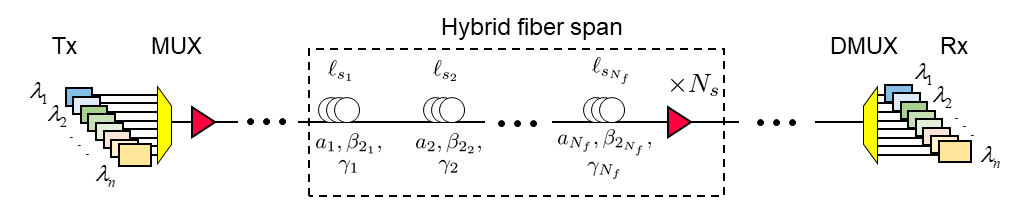
\includegraphics[scale=0.4]{BlockDiagramHybridFiberSpans_Nf.png}
\caption{Hybrid span Model}
\label{fig:hybrid_spans}
\end{figure}

\section{Stuff from Dr. Roudas}
During the AY 2019-2020, while still and undergraduate student, he took senior-level elective courses that are relevant to the scope of the project: Optical communications, Optoelectronics, and Machine learning. During the AY 2020-2021, to fulfill the MS requirements at MSU, he is taking additional telecommunications courses, i.e., Wireless communications and he is doing an Independent study in Optical Communications. This coursework is closely related to the proposed research topic and, hopefully, will help him succeed in his research goals. It is believed that, after taking these courses, the student will have acquired a solid knowledge of telecommunications and possess useful theoretical skills for doing semi-independent research on the project.

did this sync

The shutdown of the school during the second half of the Spring 2020 semester due to the COVID-19 pandemic disrupted the hiring process of foreign students for this research project. Several PhD students who were scheduled to arrive at MSU from abroad in the summer of 2020, before the start of the Fall 2021 semester, were not able to obtain student visas in time. In other cases, travel bans and the worsening pandemic forced some students to cancel or postpone their plans for graduate studies in the US. 
One of the biggest challenges the group faced during the AY 2019-2020, was restructuring the research activities of the group to a virtual format. The team is currently working in a blended fashion, both on site and remotely. MSU has a state-of-the-art high-performance computing plant. The students have remote access to the servers of this facility. It is anticipated that this facility will remain operational and the students will be able to launch simulations on hundreds of computing nodes remotely.
 
In one case, a PhD candidate who has been accepted into graduate school had to postpone the beginning of his PhD.

\section{Conclusion}
``I always thought something was fundamentally wrong with the universe'' \citep{adams1995hitchhiker}

\bibliographystyle{plain}
\bibliography{references}
\end{document}
